%%%%%%%%%%%%%%%%%%%%%%%%%%%%%%%%%%%%%%%%%%%%%%%%%%%%%%%%
%%%%                                              %%%%%%
%%%%  Author: Name des Autors                     %%%%%%
%%%%                                              %%%%%%
%%%%  Beschreibung:                               %%%%%%
%%%%                                              %%%%%%
%%%%%%%%%%%%%%%%%%%%%%%%%%%%%%%%%%%%%%%%%%%%%%%%%%%%%%%%


\chapter{Swimmer Model}
\label{chap:chapter_2}

\section{Swimmers in Nature}
\label{sec:section_1}


Biomechanical principles give the basis for understanding how a swimming body propels itself through a fluid\cite{mchenry_morphology_2005}. For example, an \textit{ascidian larva} creates
\cite{sawada_biology_2001} tail ondulation by the action of its muscles while swimming. This motion generates hydrodynamic forces and torques on the surface of the body that result in a rate and direction
of motion that are determined by body mass and its spatial distribution. A model accurately incorporating these components should successfully predict the direction, rate, and 
energetic cost of swimming.\par
Swimming bodies can be found in many different environments in the nature. The physics governing swimming in micrometer scale is other fromthe physics of swimming at the macroscopic
scale. The microorganisms are in the region of low Reynolds number, where inertia has a little effect and viscous damping is predominant. The Reynolds number is defined as:

\begin{equation} 
  Re = \frac {\rho UL}{\eta}
\end{equation}

where $\rho$ is the fluid density, $\eta$ is the viscosity and $L$ and $U$ are characteristic velocity and length scales of the flow, respectively.\par

Swimming strategies applied by large animals that run at high Reynolds number, such as fish, snakes, birds or insects\cite{childress_mechanics_1981}


are characteristic velocity and
length scales of the flow, respectively. Swimming strategies
employed by larger organisms that operate at high Reynolds
number, such as fish, birds or insects 
thesmallscale. Forexample,anyattempttomovebyimparting
momentum to the fluid, as is done in paddling, will be foiled
by the large viscous damping. Therefore microorganisms
have evolved propulsion strategies that successfully overcome
and exploit drag. The aim of this review is to explain the
fundamental physics upon which these strategies rest

\subsection{Swimming of Narrow Animals}
\label{sec:section 1}





\section{Swimmer Mechanics}
\label{sec:section 2}
The mechanics of swimmers is a complex problem\cite{tytell_interactions_2010}. The bodies of swimmers are elastic structures that deform in reaction to fluid forces but also affect the fluid around the swimmers.
In recent years, there were much progress in understanding the fluid motion around swimming bodies\cite{shadwick_fish_2006}, along with the nonlinear properties of muscle\cite{williams_new_2010} and the elastic behavior of 
swimmers bodies\cite{williams_new_2010}. Most of the studies performed with swimmers examined body mechanics separately from fluid mechanics, not including the coupled
fluid-structure interaction problem swimmers. Some Computational Fluid Dynamics (CFD) models have included some fluid-structure interaction, coupling center-of-mass motion to 
fluid dynamic forces with precribed body kinematics(\cite{kern_simulations_2006},\cite{borazjani_role_2010}).

\par

The swimmer configuration used in the simulations is described in Figure~\ref{fig:Bild1}. It is divided in three different parts: head, active tail and passive tail. The head 
is considered as an inactive region, that means no deformations are applied in the bonds belonging to it. Also, the particles that belong to the head have a lower mass property
compared to the rest of the body to represent the head flesh softness. The active tail is the beating part of the tail, the propulsion of the swimmer is generated due to sinusoidal 
propagating wave in this part of the tail. The parameters defined to describe the beat pattern will be discussed later. The passive tail has the size of 2/9 of the total tail length
and it particles has the same mass properties as the active tail, but this fragment is passive and follows the active tail beat movements. 


\begin{figure}[ht]
  \centering
  \begin{footnotesize}
  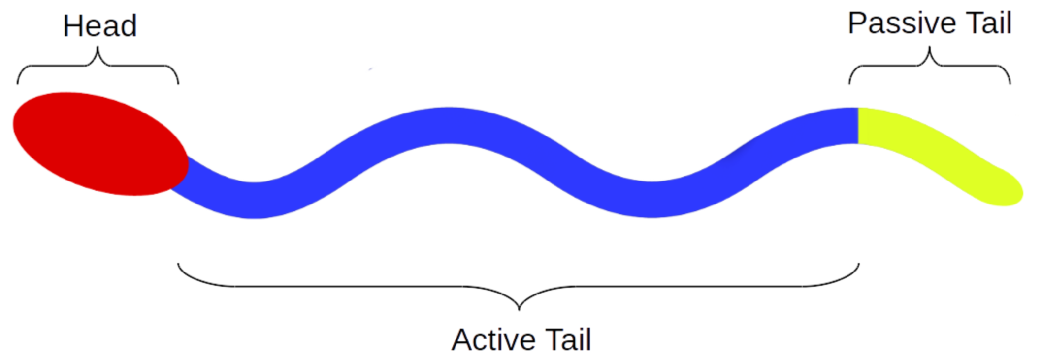
\includegraphics[scale=0.25]{images/swimmer-struc.png}
  \caption[Swimmer Structure]{Swimmer structure}
  \label{fig:Bild1}
  \end{footnotesize}
\end{figure} 


\begin{figure}
\centering
  \begin{footnotesize}
  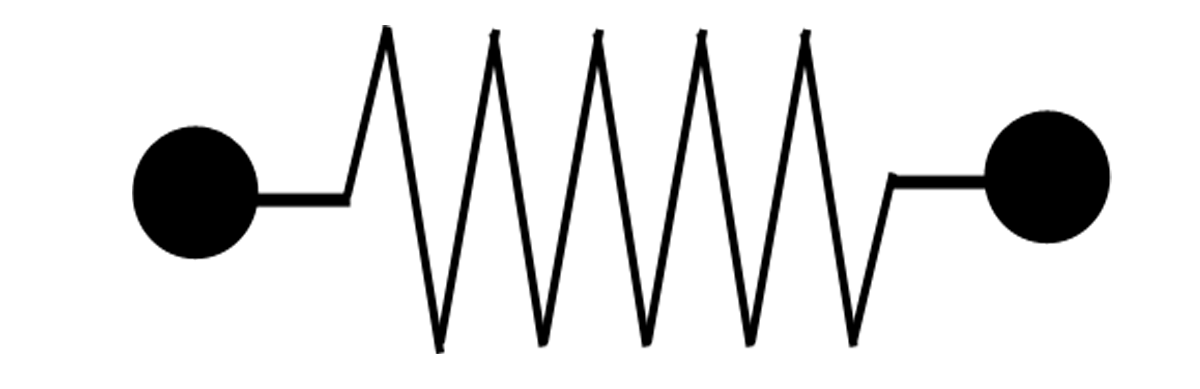
\includegraphics[scale=0.15]{images/bead-spring.png}
  \caption[Bead-Spring Structure]{Bead-Spring structure}
  \label{fig:Bild2}
  \end{footnotesize}
\end{figure} 

In this model, the swimmer consists on particles which are connected by bonds and are arranged in a filamentous structure. These particle-bonds connections have a bead-spring 
structure (Figure~\ref{fig:Bild2}). Initially, all particles in the tail ( active and passive fragments) has the same mass $m$. The bond length $l_{b}$ between neighboring
particles and the distance between the parallel filaments are identical. The filament length and the distance between filaments is described by harmonic bond potentials between
the two beads (spring constant K).\par

For the simulations, the swimmer has a total number of 100 particles, where three of those forms the swimmer head. Initially, it was used a square form for the head due to
simplifications, and after validating the method to create swimmers in LAMMPS, the swimmer was implemented with it final configuration which it is shown in Figure~\ref{fig:Bild3}.
In the final configuration the head has not a square format but an octagonal format which comes closer to the a circular/elliptical desired format. Also, when it starts to swim, 
the head takes a new format due to its mass properties, the fluid compress the head flesh turning it into a even more soft format getting closer to an ellipse and avoiding high
corner angles(Figure~\ref{fig:Bild4}).\par

\begin{figure}
\centering
  \begin{footnotesize}
  \includesvg{images/swimmer-compare-final}
  \caption[Initial swimmer structure configuration (upper) and modified final swimmer structure (lower)]{Initial swimmer structure configuration (upper) and modified final swimmer structure (lower)}
  \label{fig:Bild3}
  \end{footnotesize}
\end{figure} 

\begin{figure}
\centering
  \begin{footnotesize}
  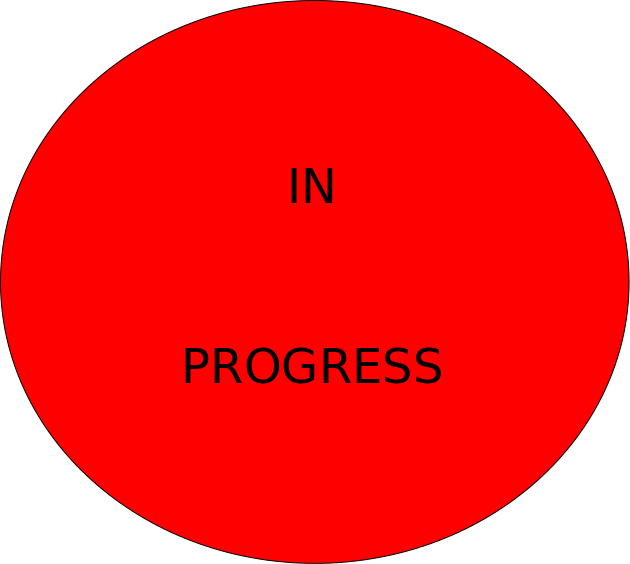
\includegraphics[scale=0.25]{images/in-progress.png}
  \caption[inprogress]{inprogress}
  \label{fig:Bild4}
  \end{footnotesize}
\end{figure} 

The harmonic bonds used to create the connections between the swimmer particles are applied in different ways thru the swimmer.Bonds are defined between specified pairs of 
atoms and remain in force for the duration of the simulation (unless the bond breaks which is possible in some bond potentials). The harmonic bond style uses the potential:


\begin{equation} 
  E = K ( r - r_{0})^2
\end{equation}

where $r_{0}$ is the equilibrium bond distance and $K$ is the bond stiffness constant. Note that the usual $1/2$ factor is included in $K$.

The internal bonds of the swimmer, that means the bonds which connects the upper and lower lines of the structure, have the aim to represent the swimmer backbones, so its 
physiological properties are different, and to represent it, the stiffness of those bonds are higher then the others in the swimmer borders. The passive bonds present in the 
rear of the tail are also harmonic and their lengths $l_{b}$ are constant. The active tail is formed by two lines of atoms connected by bonds, an upper and a lower line. Those
lines have a different bond type compared with the rest of the swimmer, as they are called active, the bond length is not constant in time. Changing the bond length it generates
a local spontaneous curvature. A sinusoidal variation of the bond length as a function of the contour length and time then generates the sinusoidal propagating wave of the active
lines. This approach is the most common in literature models, to prescribe the swimmer motion.\par

In Figure~\ref{fig:Bild5}, the red lines show the internal bonds with a higher stiffness relative with the rest of the swimmer, the blue points connected by the blue line show the 
head flesh which has an smaller mass and gets deformed as it swimms.\par
Many changes were applied in LAMMPS code as it was not ready to create specifically swimmers. Those changes are shown in the Chapter 3.


\begin{figure}
\centering
  \begin{footnotesize}
  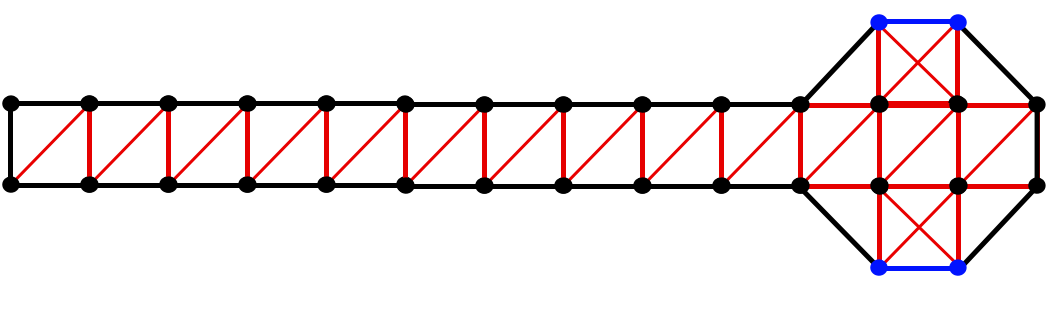
\includegraphics[scale=0.25]{images/swimmer-compare.png}
  \caption[Structure of the swimmer describing the internal bonds (red), the swimmer surface bonds (black) and the head flesh particles and bonds(blue)]{Structure of the swimmer describing the internal bonds (red), the swimmer surface bonds (black) and the head flesh particles and bonds (blue)}
  \label{fig:Bild5}
  \end{footnotesize}
\end{figure} 




